\subsection{RQ2: What factors impact the difficulty of a conflict resolution?}\label{RQ2}

\todo{talk about resolution difficulties in interviews and how survey answer options were formed}

Our survey suggests that regardless of gender, developer role, experience level, project size, and source distribution model, software practitioners say that the following factors affect the difficulty of resolving merge conflicts: 
\begin{itemize}
\item \textit{The amount of information you have about the conflicting code}\\
\item \textit{Your expertise in the area of code with the merge conflict}\\
\item \textit{How easy it is to understand the code involved in the merge conflict}\\
\item \textit{How well tools present information in an understandable way}
\item \textit{Complexity of the project structure}
\end{itemize}

Nothing is considered to have no effect on merge conflict resolution difficulty

21-25 stands out, but it could be due to low sample sizes

Tool support history and informativeness of commit messages are both controversial across project sizes.

Trustworthiness of tools is controversial across experience levels

Project culture, Tool support history, Informativeness of commit messages are controversial across all demographics

Trustworthiness of tools is controversial across different roles.

Project culture becomes more impactful as project size increases.

Trustworthiness of tools: Sys Architects, Sys Admins, and Project Managers say it has an effect. Sys Engineers and Project Maintainers say it has no effect. This could be because people who are closer to the code have found their tools and have settled into their processes. They know the workarounds, and they have done this before.

\textbf{***Tool support for examining development history from 10th to 1st***}\\
\textbf{***Expertise in the area of code becomes less important (1-4) ***}\\
\textbf{***Project Culture generally not important, especially with more experience***}\\
\textbf{***commit message informativeness lower than expected***}\\

%\begin{figure}[!t]
%\centering
%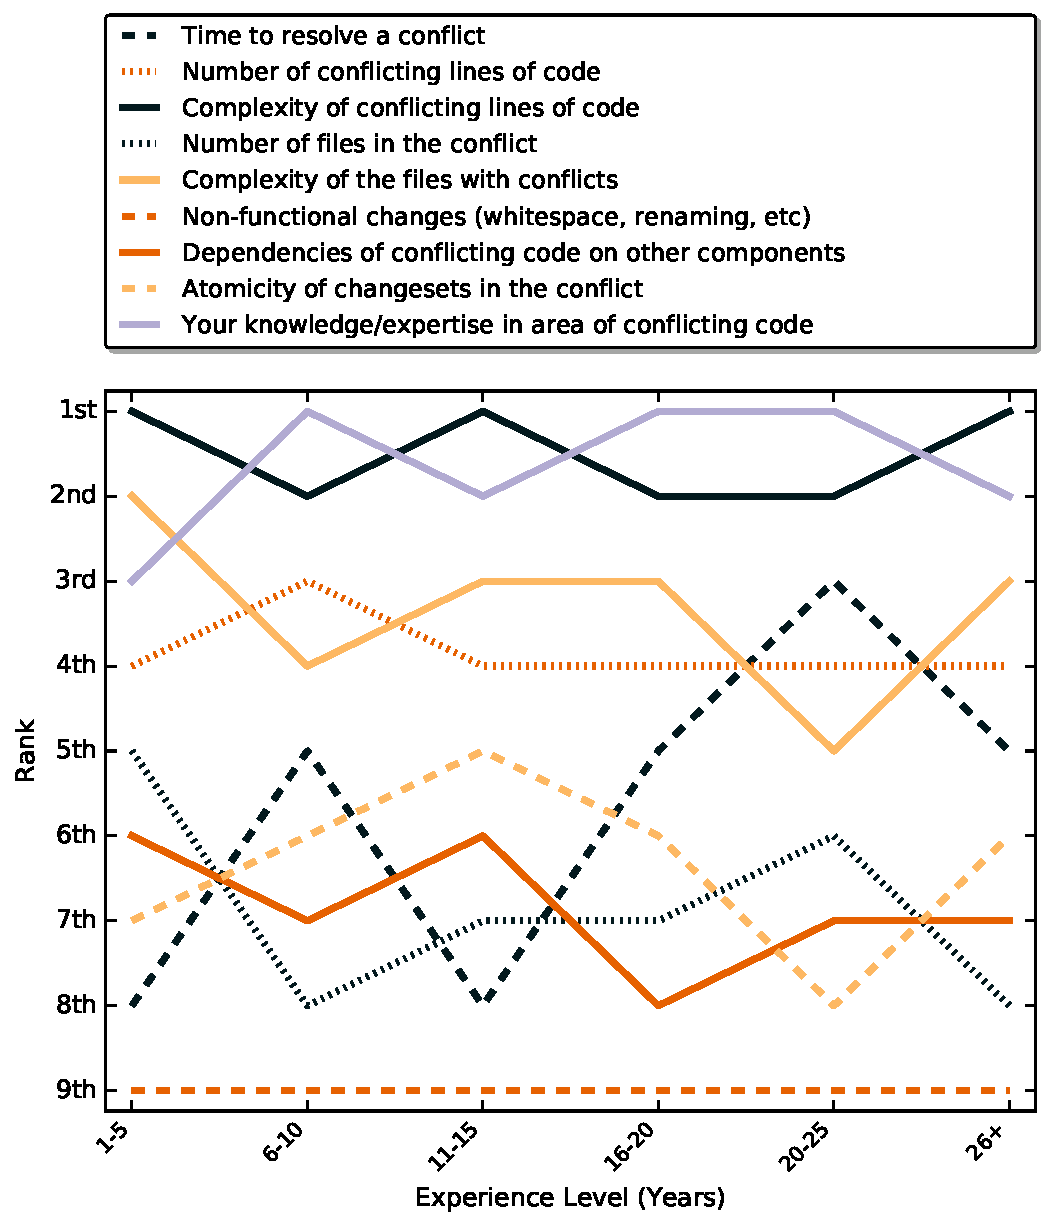
\includegraphics[width=2.5in]{ExpVsRankConDiff.pdf}
%\caption{Rank of difficult factors in merge conflicts by experience level}
%\label{con_diff_rank}
%\end{figure}